\chapter{Implementierung}
\label{Kap5}
Die zuvor herausgearbeiteten Konzepte werden nun im bereits vorhandenen Webportal umgesetzt. Dabei wird der bisherige Aufbau der Anwendung analysiert und erweitert. Einzelne wichtige Aspekte werden in diesem Kapitel herausgegriffen und erläutert.

\section{Offline Metadaten}
Jeder Inhalt auf CROSSLOAD besitzt Eigenschaften, die hier als Metadaten bezeichnet werden. Dazu gehören zum Beispiel die Id, Titel, Bibelstellen, Ort oder Datum. Diese Metadaten werden benötigt, um Suchergebnisse oder die Detailseite einer Predigt anzuzeigen. In diesem Kapitel werden Strategien beschrieben, wie diese Metadaten gecached werden, um eine bestmögliche Nutzererfahrung zu bieten.

\subsection{Detailseite}
Im Webportal CROSSLOAD wird bereits ein Service Worker verwendet, der einerseits statische Inhalte zwischenspeichert aber auch dynamische Requests cached. Für dynamische Requests wurde bislang die Cache Strategie freshness verwendet. Das heißt, dass der Cache nur verwendet wird, wenn die Netzwerkanfrage fehlschlägt \autocite{angular-service-worker}. Die momentane Lösung ist nicht optimal. Sie ermöglicht zwar eine Offlineverfügbarkeit der Daten aber bietet nicht die optimale Geschwindigkeit für den Nutzer. In vielen Fällen wird sich der Inhalt im Cache nicht mit der Antwort aus der Netzwerkanfrage unterscheiden, trotzdem muss der Nutzer auf die Antwort vom Netzwerk warten. Eine bessere Lösung ist folgende:

Wenn der Nutzer einen Inhalt auswählt, wird direkt im Cache nachgeschaut, ob dieser Inhalt bereits existiert. Sofern er existiert, wird er dem Nutzer angezeigt. Gleichzeitig wird eine Netzwerkanfrage geschickt. Sobald die Antwort vom Netzwerk ankommt, wird die Antwort mit dem Wert im Cache verglichen. Wenn sich die Werte unterscheiden, wird der Cache aktualisiert und dem Nutzer werden die aktuelleren Daten angezeigt. Diese Strategie ist mit Service Workern nicht allzu einfach zu lösen, weil ein Service Worker nur ein Mittelsmann in einem Request ist. Das heißt, er kann nur einen einzigen Wert zurückgeben und nicht einen zweiten etwas zeitverzögert. Deswegen werden die Metadaten nicht im Service Worker gecached, sondern in einem Angular-Service.

\bild{diagramme/inhalt-sequenzdiagramm}{14cm}{Sequenzdiagramm für den Abruf der Metadaten eines Inhalts}

In \autoref{diagramme/inhalt-sequenzdiagramm} ist die bereits beschriebene Cache-Strategie gezeigt. Alle Teile in Schwarz sind bereits vorhanden. Die Teile in Rot sind Ergänzungen im Rahmen dieser Arbeit. Im ContentService werden bereits Subjects und Observables verwendet. Durch das Publish-Subsribe Pattern, das dadurch erzeugt wird, ist es möglich, mehrere Subscriber (in diesem Fall nur ContentPage) zu benachrichtigen, sobald sich ein Inhalt ändert. Darüber hinaus ist es auch möglich, etwas zeitversetzt einen aktualisierten Inhalt auszuliefern. Der OfflineService verwaltet den Cache, dessen Implementierung wird in \autoref{Kap5:Speicherung} genauer beschrieben. Manche Metadaten des Inhalts werden nur lokal gespeichert. Dazu gehört beispielsweise, ob ein Inhalt favorisiert ist und ob die entsprechende Audiodatei offline verfügbar ist. Deswegen werden die Metadaten vom Backend mit den Metadaten aus dem OfflineService erweitert.

\subsection{Suche}
Auf CROSSLOAD ist es möglich, Inhalte anhand verschiedener Kriterien zu suchen. Die Suche wird dabei nicht gecached, was auch weiterhin so bleiben soll. Die Suchergebnisse können sich oft ändern, zum Beispiel wenn neue Inhalte hinzukommen, sodass sich ein cachen der Ergebnisse nicht lohnen würde. Dem Nutzer soll allerdings trotzdem angezeigt werden, ob ein Inhalt, der in der Suche angezeigt wird, bereits offline verfügbar oder favorisiert ist. Dafür muss für jeden Inhalt aus den Suchergebnissen im Offline-Speicher nachgeschaut werden, ob der Inhalt dort verfügbar ist. Diese Überprüfung kann je nach Anzahl der Inhalte einige Millisekunden dauern. Um die bestmögliche Nutzererfahrung bieten zu können, wird eine ähnliche Strategie wie für die Detailseite verwendet:

\bild{diagramme/suche-sequenzdiagramm}{14cm}{Sequenzdiagramm für die Suche nach Inhalten}

In \autoref{diagramme/inhalt-sequenzdiagramm} wird der Ablauf für das Suchen auf CROSSLOAD dargestellt. Alle Teile in Schwarz, sind bereits vorhanden und die Teile in Rot sind Ergänzungen im Rahmen dieser Arbeit. Sobald ein Nutzer Inhalte auf CROSSLOAD sucht, wird eine Netzwerkanfrage gesendet. Sobald die Antwort der Anfrage da ist, werden dem Nutzer die Inhalte angezeigt. Gleichzeitig wird für jeden gefundenen Inhalt überprüft, ob er bereits offline verfügbar ist. Dieser Status wird dann in das Suchergebnis geschrieben. Sobald alle Inhalte überprüft wurden, werden dem Nutzer die aktualisierten Suchergebnisse angezeigt. Dafür wird wieder das Publish-Subscribe Pattern verwendet. 

\section{Lokale Datenspeicherung}
\label{Kap5:Speicherung}
Für die Speicherung von Offline-Daten wurde sich bereits für IndexedDB entschieden. Die Verwendung von IndexedDB ist nicht trivial, weil mit Events gearbeitet wird und nicht wie in moderneren APIs mit Promises \autocite{mdn-indexeddb}. Es gibt aber einige Bibliotheken, die das Arbeiten mit IndexedDB erleichtern. Für diese Arbeit wurde Dexie.js ausgewählt. Dexie.js ist ein minimaler Wrapper für IndexedDB, zum Arbeiten mit Promises \autocite{dexie}. Es gibt auch noch andere Bibliotheken wie beispielsweise LocalForage. Dexie wurde jedoch ausgewählt, weil mehrere Indexe in der Datenbank unterstützt werden. Generell ist die Bibliothek sehr flexibel und trotzdem klein.

Die ganze Logik befindet sich in der Angular-Anwendung in einem Service. Dieser Service abstrahiert alle Datenzugriffe, sodass, falls später notwendig, Dexie auch durch eine andere Bibliothek ausgetauscht werden kann. 

IndexedDB besitzt kein Schema, wie von relationalen Datenbanken bekannt. Es können beliebige Objekte gespeichert werden, die nicht alle die gleiche Struktur besitzen. Wenn man diese Objekte aber durchsuchen möchte, sollte man jedoch einen Index auf die durchsuchten Eigenschaften legen. Diese Indexe muss man beim Erstellen der Tabellen angeben. Für diese Anwendung werden zwei Tabellen angelegt: \emph{favoriten} und \emph{downloads}. Siehe auch \autoref{architekturen/architektur-indexed-db} zur Erklärung.

Die Tabelle \emph{favoriten} enthält alle Metadaten zu einem Inhalt. Für diese Daten besteht bereits ein Datenobjekt, welches in der Datenbank gespeichert wird. Als Index wird vorerst nur die \emph{Id} des Inhalts festgelegt. Später, wenn auch nach anderen Kriterien gesucht oder gefiltert werden soll, kann ein weiterer Index hinzugefügt werden. 

Die Tabelle \emph{downloads} speichert die Audiodateien. Als Schlüssel dient dazu die Id des Inhalts. Auf dieser Id liegt ein Index, damit schnell eine Audiodatei zu einem favorisierten Inhalt geladen werden kann.

\section{Herunterladen der Audiodaten}
Auch das Herunterladen der Audiodaten wird in einem Angular-Service umgesetzt. Der Service ist dafür zuständig abzufragen, welche APIs auf dem aktuellen Gerät unterstützt werden und startet dann den Download. Zuerst wird das Herunterladen mittels dem HttpClient von Angular implementiert. Eine zusätzliche Implementierung von Background Fetch ist in dieser Arbeit nicht vorgesehen, aber für zukünftige Entwicklungen von CROSSLOAD vorgemerkt. 

\autoref{diagramme/download-sequenzdiagramm} zeigt die Benutzung des \textit{DownloadService} zusammen mit anderen Komponenten. Dazu gehört die \textit{ContentPage}, welche dafür zuständig ist, einen Inhalt anzuzeigen. Über die \textit{ContentPage} kann ein Inhalt favorisiert und heruntergeladen werden. Der Downloadfortschritt soll an mehreren Stellen in der Anwendung verfügbar sein: Der Download soll auf der entsprechenden \textit{ContentPage} angezeigt werden. Außerdem gibt es eine \textit{DownloadComponent}, welche alle laufenden Downloads mit Fortschritt anzeigt. 

Auch der \textit{DownloadService} setzt wieder auf Subjects und Observables, um das Publish-Subscribe Pattern umzusetzen. Zuerst wird ein Subject erzeugt, über das später der Downloadfortschritt an andere Komponenten geschickt wird. Immer wenn ein Fortschritt vom \textit{HttpService} kommt, wird dem Subject ein neuer Wert geschickt. Die \textit{ContentPage} abonniert Ergebnisse auf dem Subject, die etwas mit dem Inhalt zu tun haben, der gerade angezeigt wird. Die \textit{DownloadComponent} dagegen abonniert alle Fortschritte. Sobald ein Download fertiggestellt wurde, wird ein letztes mal ein Fortschritt versendet und das Ergebnis über den \textit{OfflineService} in die IndexedDB im Browser abgelegt.

\begin{sidewaysfigure}
 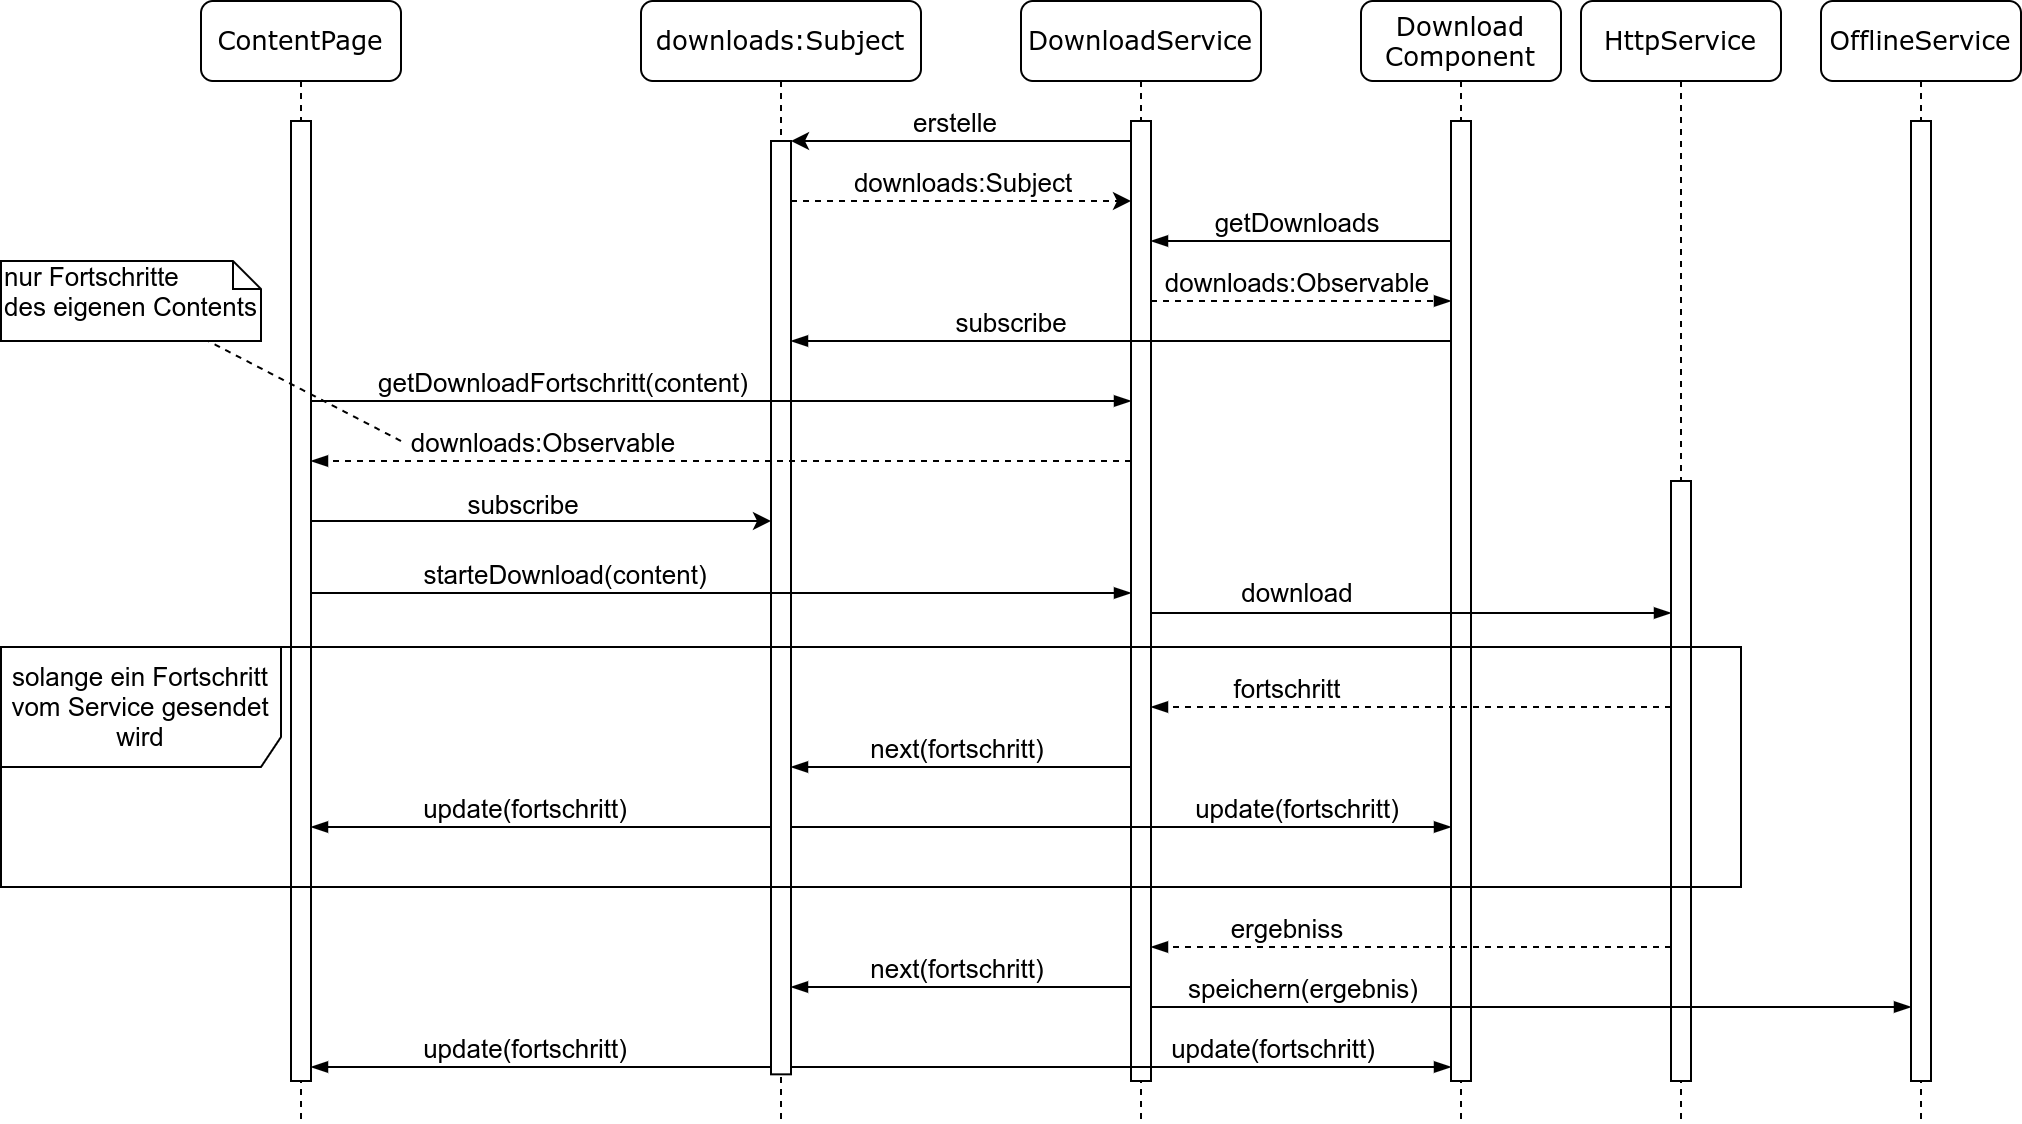
\includegraphics[width=22cm]{diagramme/download-sequenzdiagramm}
  \caption{Sequenzdiagramm für den Download von Dateien}
  \label{diagramme/download-sequenzdiagramm}
\end{sidewaysfigure}

\section{Grafische Oberfläche}
Der Designentwurf für die Funktion \textit{unterwegs anhören} wurde gemeinsam mit den Mitarbeitern von CROSSLOAD diskutiert und herausgearbeitet. 

In der Desktop-Ansicht wird in den Player ein Switch hinzugefügt, mit dem ein Inhalt offline verfügbar gemacht werden kann. In \autoref{designs/player} ist dieser Player mit dem Button zu sehen. Außerdem existiert ein Button \textit{Meine Inhalte}, mit dem man auf die Übersichtsseite mit allen heruntergeladenen Inhalten kommt.

\bild{designs/player}{14cm}{Player der Desktop-Ansicht}

Da der Player in der mobilen Ansicht nicht genügend Platz bietet, wird der Switch zum Herunterladen hier unter dem Player dargestellt. Dies ist in \autoref{designs/player-mobile} zu sehen. Wenn der Player vergrößert wird, erscheint zusätzlich der Button \textit{Meine Inhalte}, wie in \autoref{designs/player-mobile-gross} zu sehen.

\bild{designs/player-mobile}{8cm}{Design: Player der mobilen Ansicht}

\bild{designs/player-mobile-gross}{8cm}{Design: ausgefahrener Player der mobilen Ansicht}

Zuletzt zeigt \autoref{designs/uebersicht} eine Liste mit allen Inhalten, die heruntergeladen wurden. Diese können einzeln oder alle auf einmal gelöscht werden. Außerdem ist es möglich, einen Inhalt abzuspielen oder alle heruntergeladenen Inhalte zu durchsuchen.

\bild{designs/uebersicht}{8cm}{Design: Liste mit allen heruntergeladenen Inhalten}